\section{Applications}
\label{sec:apps}

In the previous sections, we described the goals of various applications
and motivated why it was difficult to accomodate them in the standard
web architecture.  Then, we described the \sys{} system, explaining the
primitives we introduced to the browser.  In this section, we close the
loop, explaining how to use this primitives to implement the
applications described in the first section.

\subsection{Encrypted Document Editor}

In the previous section, we described the key feature needed by an
encrypted document editor: symmetric confinement, where two mutually
distrusting scripts can confine each other's use of data that has been
sent.  The key to implementing this application will be judicious use of
\emph{privileges}, which are asymmetrically distributed to the
distrusting components.

\begin{figure}
\centerline{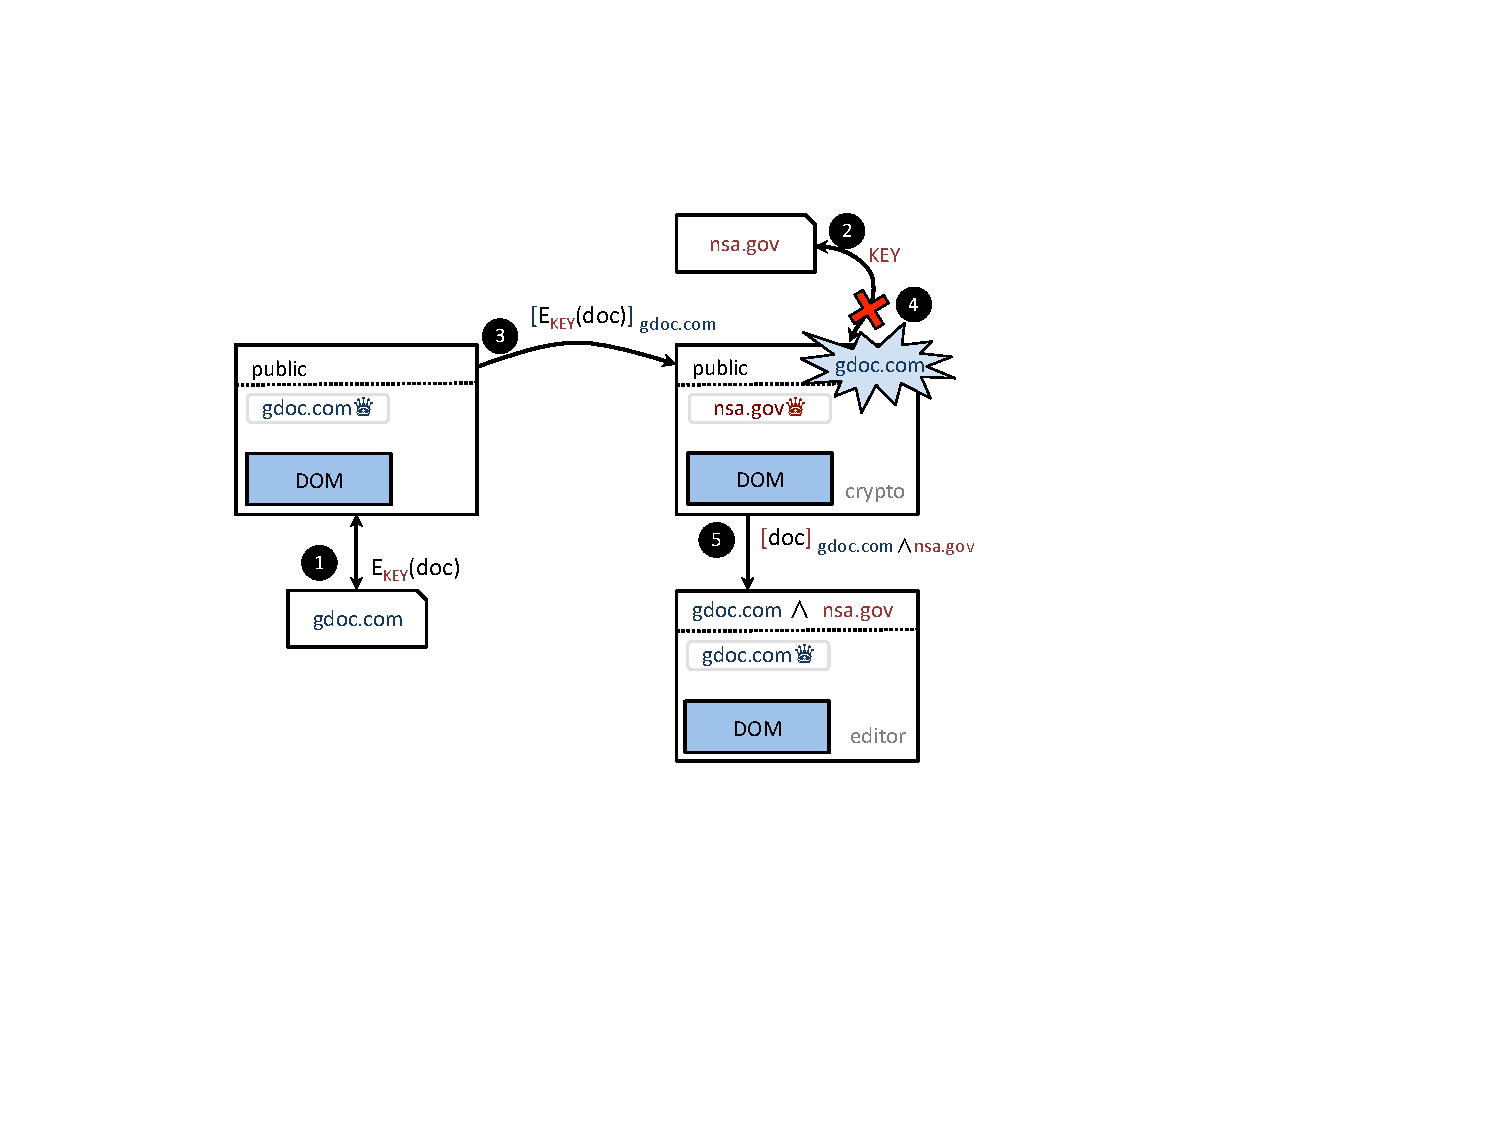
\includegraphics[width=\columnwidth]{editor}}
\caption{\label{fig:editor} Encrypted document editor architecture
under \sys{}.}
\end{figure}

In Figure~\ref{fig:editor}, the architecture for an encrypted document
editor is shown.  The editor has three components: a component which has
your Google Documents credentials and communicates with the server (\https{gdoc.com}), the
editor proper (also \https{gdoc.com}), and the component which performs encryption (\https{nsa.gov}).  We give the
following security guarantee: if the \https{nsa.gov} is honest, then we
guarantee that the clear text of your document is never leaked to any
origin.  If only \https{gdoc.com} is honest, then \https{gdoc.com} may
be able to recover your cleartext (e.g.\ the encryptor used the null
cipher), but the encryptor should not able to exfiltrate the cleartext
to anyone else.

What occurs when you open Google Documents to edit an encrypted
document?
%
Initially, \https{gdoc.com} downloads (1) the encrypted document from
Google's servers.
%
Seeing that the document is encrypted, it opens an iframe to
\https{nsa.gov}, exercising its privilege to keep its initial label as
\https{nsa.gov} so it can talk to the \https{nsa.gov} server and
download the private key (2) which will be used to decrypt the document.
%
Next, it sends the encrypted document as a labeled blob, with the label
``\https{gdoc.com}'' (3); the iframe raises its label (4) so it can read
and decrypt the document.
%
Finally, the iframe passes on the decrypted document (labeled as
``\https{gdoc.com} and \https{nsa.gov}'') to a new iframe (5) which
implements the editor proper.

To save the document, we run this flow in reverse: the editor sends a
decrypted document to the encryptor (5), which encrypts it with the
private key.  Next, the critical step occurs: the encryptor exercises its privileges
to send a labeled blob of the encrypted document which is \emph{only}
labeled \https{gdoc.com} (3).  Since the encryptor is the only compartment
with the \https{nsa.gov} privilege, all documents must pass through it for
encryption before being sent out to the world; conversely, it itself cannot
exfiltrate any data, as it is operating with \https{gdoc.com} in its label.

One interesting thing to note about this architecture is that a user can
verify that Google Documents appropriately loaded the encryptor, since
without it, it would not be possible to display the decrypted text.  However, when
a new document is being created, the encryptor iframe must be placed
in a separate pop-up window, so that the user can verify that encryption
has been enabled.\footnote{This architecture might be desirable in any case
to prevent phishing.}

Due to space limitations, we do not discuss the architecture of the
password manager we built in detail; however, it operates on very
similar principles to the encrypted document editor.

\subsection{Third-Party Mashup}
\label{sec:apps-mashup}

\begin{figure}
\centerline{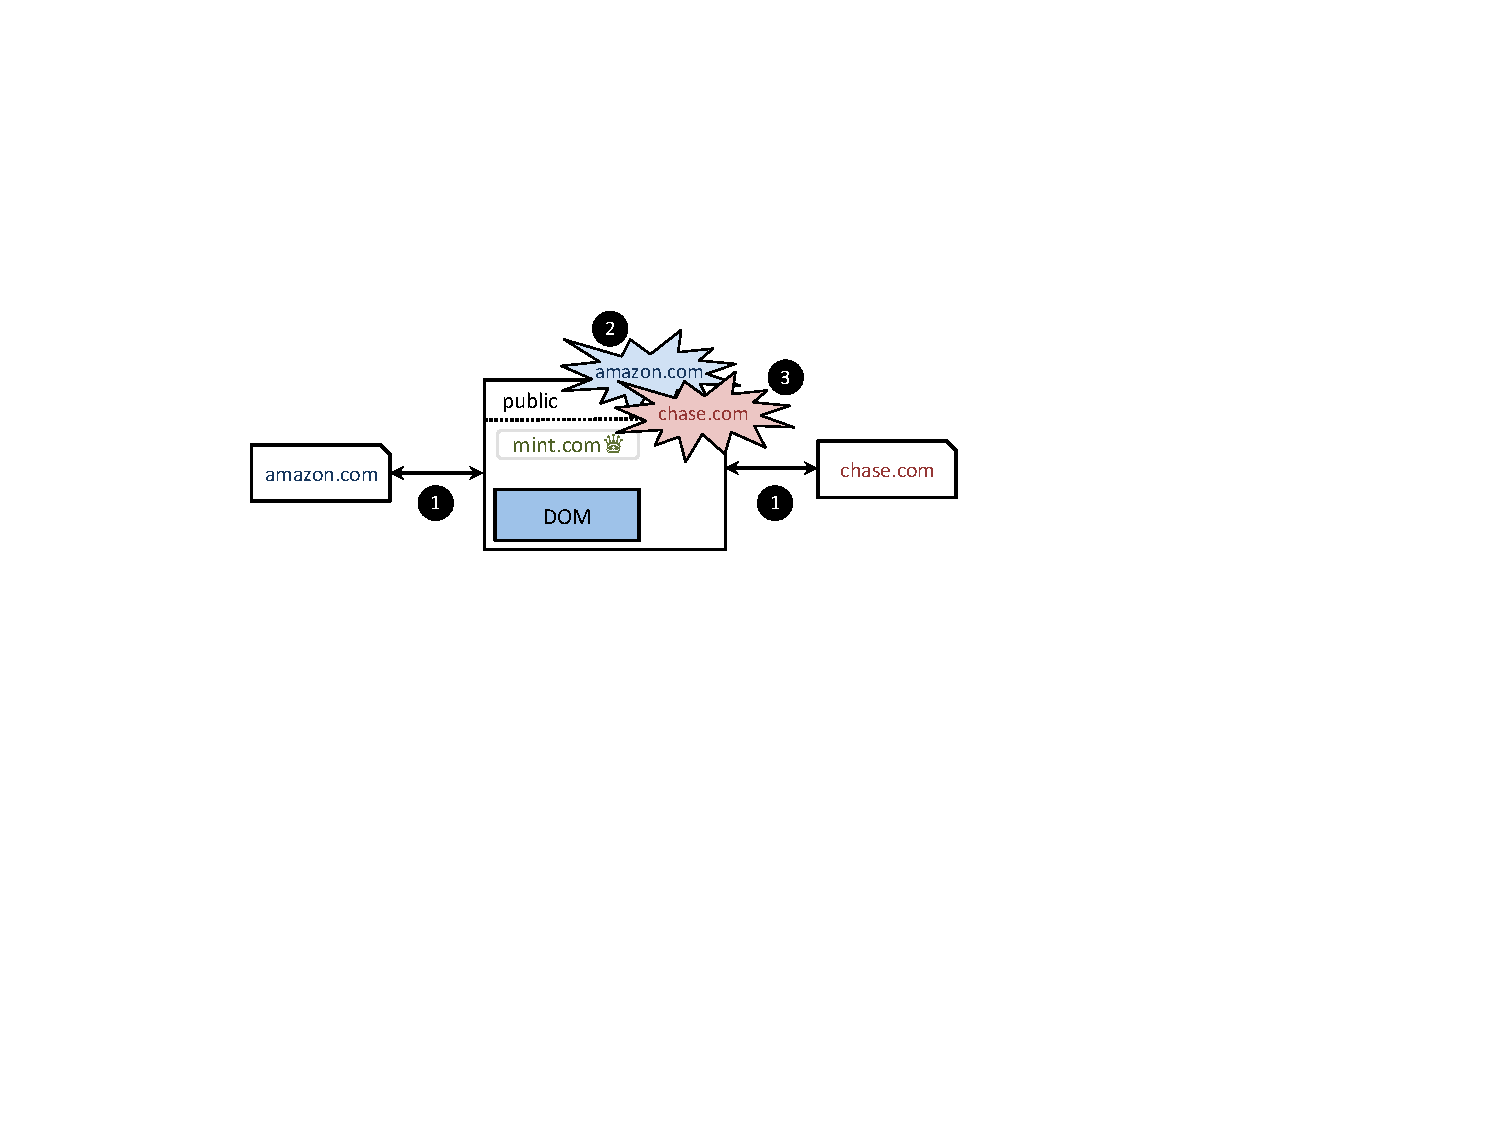
\includegraphics[width=\columnwidth]{mashup}}
\caption{\label{fig:mashup} Third-party mashup under \sys{}.}
\end{figure}
The key feature that enables us to build third-party mashups is
labeled XHR\@.  In Figure~\ref{fig:mashup}, the architecture for an
application which reconciles a user's Amazon purchases
and bank statement is shown.  As opposed to the encrypted document editor,
the architecture for this mash-up is very simple: we just download
information from a few websites, and then do some computation on them.

It's instructive to consider a version of this mash-up which does not
work.  Suppose that we use regular XHR in order to retrieve data from
\https{chase.com} and \https{amazon.com}.  Ordinarily, we cannot read
the results of XHR, since \https{chase.com} does not flow to \https{mint.biz}.
We might change our label to be \https{chase.com} (exercising the \https{mint.biz}
privilege), but now we cannot contact \https{amazon.com}.

Labeled XHR (Section~\ref{sec:labeled-xhr}) provides a solution to
this conundrum.  First, we make labeled XHRs to both web sites (1),
maintaining our current label but receiving labeled blobs.  Once all of
the information is received, we raise our current label (2--3) and
unlabel the blobs, in the process restricting our communication to the
web at large.

\subsection{Untrusted Third-Party Library}
\label{sec:apps-third-party}

\begin{figure}
\centerline{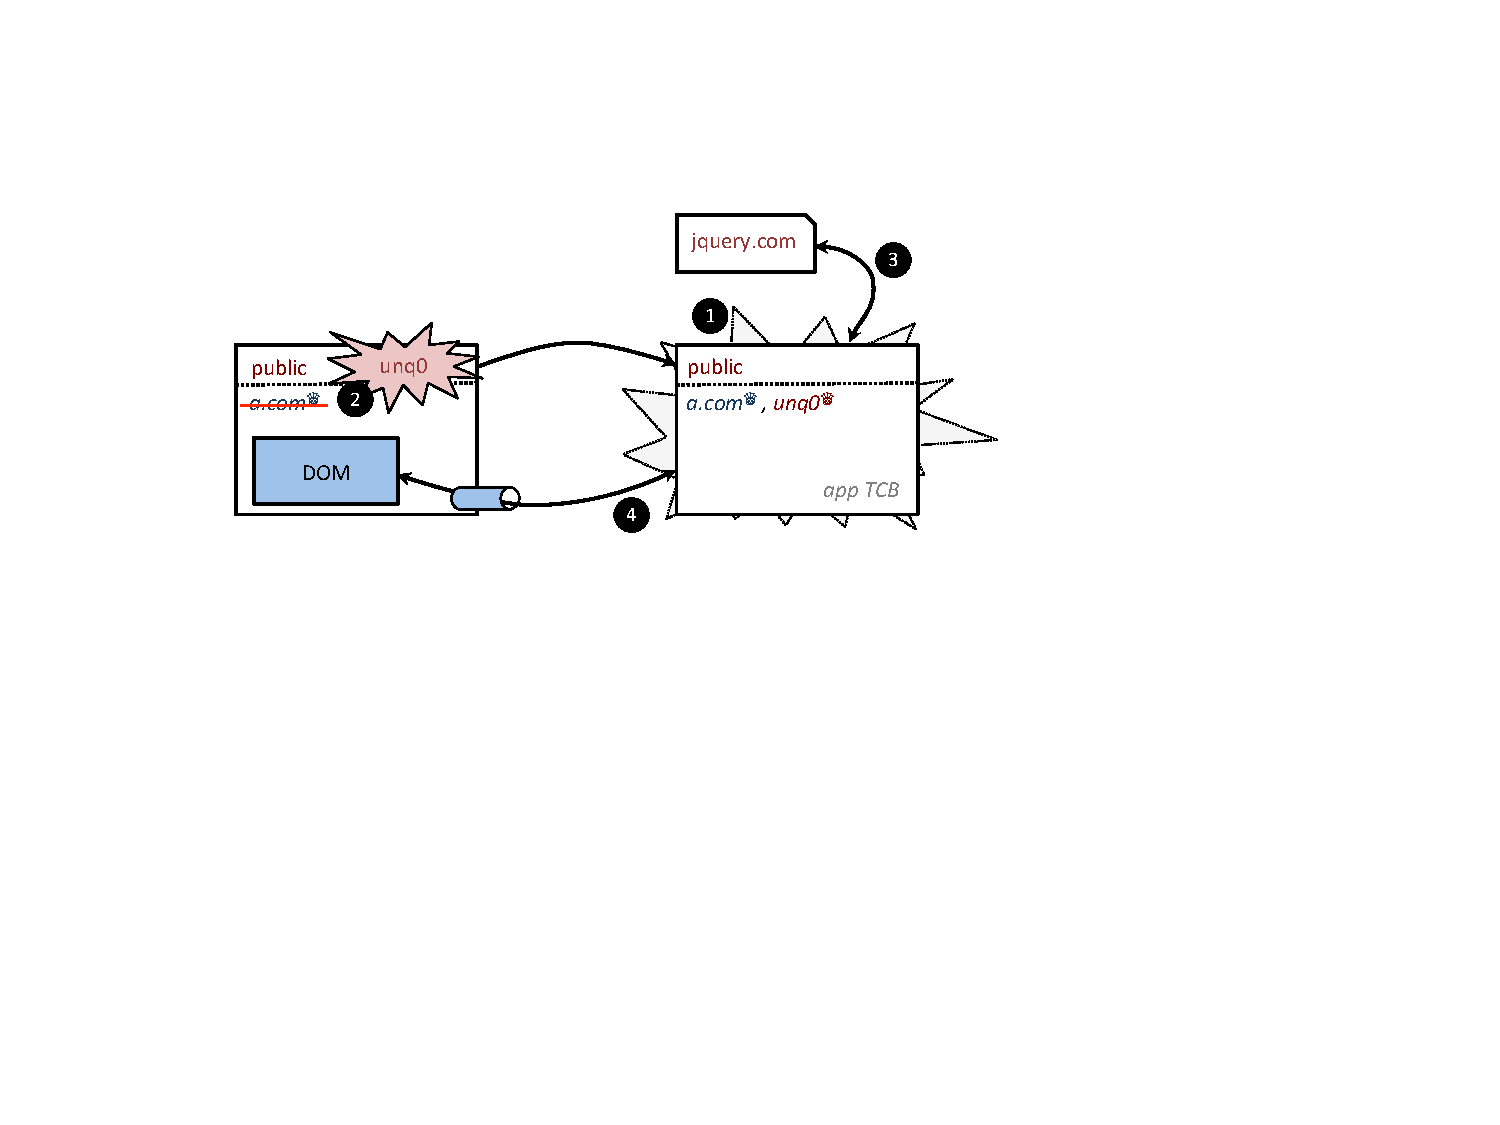
\includegraphics[width=\columnwidth]{jquery}}
\caption{\label{fig:mashup} Privilege separation and library
confinement in \sys{}.}
\end{figure}

The key feature that lets us confine untrusted third-party libraries
like jQuery is the ability to place trusted code in another context,
which can access the main page but \todo{ar}{what do you mean by vice-versa?} not vice-versa.

In Figure~\ref{fig:jquery}, the architecture for a web page using an
untrusted JavaScript library is shown.  Our goal is to establish a
separate DOM worker which has the \https{a.com} privilege, while the
main browsing context runs jQuery without privileges or the ability to
talk to the network.  Initially, we start in the main browsing context
with the \https{a.com} privilege.  We generate a fresh privilege/origin
pair, and spawn a DOM worker (1), delegating both privileges to it.  The
main context drops both privileges (2), while both compartments raise
their label to ``\https{a.com} and fresh-privilege'' (3).  Finally, the
trusted worker downloads jQuery (4) and passes the script contents to
the main context, which loads the library (5).  At the time the library
is loaded, the main context becomes untrusted, but this is no matter, as
it is fully confined at this point.  As the trusted DOM worker has both
privileges, it can freely modify the DOM of the main context, as well as
communicate with the wider web.  We can think of this DOM worker as a
\emph{firewall} between the page proper (with the untrusted library)
and the rest of the world.
\todo{ar}{If JQuery needs to use the network, then it need to ask for that to 
the worker, right?}
